\documentclass[floatfix,prb,aps,superscriptaddress,showpacs,11pt,preprint,letterpaper]{revtex4}
\usepackage{amsmath}
\usepackage{graphicx}
\usepackage[backref,pdffitwindow,colorlinks,linkcolor={blue},citecolor={red}]{hyperref}
\def\chon{red}
%\usepackage{showlabels}

\pacs{78.68.+m, 42.65.An, 71.15.Mb, 42.65.Ky, 78.66.-w}

\begin{document}

\title{Theory of surface second-harmonic generation for 
       semiconductors including effects of nonlocal operators}

\author{Sean M. Anderson}
    \affiliation{Centro de Investigaciones en Optica, 
                Le\'on, Guanajuato, M\'exico}
\author{Nicolas Tancogne-Dejean}
    \affiliation{Laboratoire des Solides Irradi\'es, \'Ecole Polytechnique, 
                CNRS, CEA/DSM, 91128 Palaiseau, France}
    \affiliation{European Theoretical Spectroscopy Facility (ETSF), 
                Palaiseau, France}
\author{Bernardo S. Mendoza}\email{bms@cio.mx}
    \affiliation{Centro de Investigaciones en Optica, 
                Le\'on, Guanajuato, M\'exico}
\author{Val\'erie V\'eniard}
    \affiliation{Laboratoire des Solides Irradi\'es, \'Ecole Polytechnique, 
                CNRS, CEA/DSM, 91128 Palaiseau, France}
    \affiliation{European Theoretical Spectroscopy Facility (ETSF), 
                Palaiseau, France}

\begin{abstract}
We formulate a theoretical approach of surface second-harmonic generation 
from semiconductor surfaces based on the length gauge and the 
electron  
density operator.  
Within the independent particle approximation 
the nonlinear second-order surface susceptibility tensor
$\chi^{\mathrm{a}\mathrm{b}\mathrm{c}}(-2\omega;\omega,\omega)$    
is calculated, including for the first time in one unique formulation
(i) the scissors correction, needed to have the correct value of the
energy band gap,
(ii) the contribution of the nonlocal part of the  
pseudopotentials, routinely  used in \textit{ab initio} band structure calculations, 
and (iii) the derivation for the inclusion of the cut function, 
used to extract the surface response.
The first two contributions
are described by spatially nonlocal quantum
mechanical operators and are fully taken into account in the present formulation. 
As a test-case of the approach we calculate 
$\chi^{xxx}(-2\omega;\omega,\omega)$ for the clean Si(001)$2\times 1$
reconstructed surface and find that our scheme to extract the surface
through the cut function
readily works and is exact. The effects of the scissors correction and
of the nonlocal part of the pseudopotentials are discussed 
in surface nonlinear optics. 
The scissors correction shifts the spectrum to 
higher energies though the shifting is not rigid and mixes the 
$1\omega$ and $2\omega$ resonances, 
and has a strong influence in the line-shape. 
The 
effects of the nonlocal part of the pseudopotentials 
keeps the same line-shape of $|\chi^{xxx}_{2\times 1}(-2\omega;\omega,\omega)|$, but 
reduces its value
by 15-20\%.  
Therefore, the inclusion of the three aforementioned 
contributions is very important and 
makes our scheme unprecedented and opens the possibility to 
study surface second-harmonic generation
with more versatility and providing more accurate results.
\end{abstract}  

\maketitle

\section{Introduction}\label{intro}

In recent years surface nonlinear optical spectroscopies, particulary surface 
second-harmonic generation (SSHG), have evolved as useful nondestructive 
and noninvasive tools to study surface and interface properties. These 
properties include atomic structure, phase transitions, adsorption of 
atoms, and many others.\cite{daumPRL93, mcgilpOE94, meyerPRL95, powerPRL95, 
godefroyAPL96, hoferAPA96, dadapPRB97, bloembergenAPB99, mcgilpSRL99, 
suzukiAPB99, mitchellSS01, hughesPRB96, guyotPRB88, downerPSSA01, shenAPB99, 
shenNAT89, chenPRL81, mendozaPRL98, downerSIA01} Nowadays, SSHG spectroscopy 
is a crucial tool for research and development in microelectronics,
\cite{zheltikovLP00} semiconductors, \cite{lupkeSSR99} nanomaterials,
\cite{salazar-aparicioPRB14} and many more recent areas of great scientific 
and commercial interest.\cite{cazzanelliNM14} The high surface sensitivity 
of SSHG spectroscopy is due to the fact that within the dipole approximation 
the bulk SHG signal of centrosymmetric materials is identically zero.
Radiation can occur only at the surface where the inversion symmetry is 
broken. 
The bulk quadrupole contribution for centrosymmetric materials is
different from zero, but usually it is very small,\cite{downerSIA01} and we neglect it. 
Much of the foundation of surface science has been built from 
experiments involving emission or scattering of electrons from surfaces. 
These require ultrahigh vacuum (UHV) environments and provide no access to 
buried interfaces. However, SSHG is compatibile with non-UHV conditions and 
has access to interfaces buried beneath transparent overlayers. Even when 
applied to surfaces in UHV, the light source and detectors can be aligned and
used outside the vacuum chamber. 

The usefulness of SSHG could be limited by the lack of microscopic theoretical
understanding of the nonlinear spectra. The macroscopic phenomenological 
theory of SSHG, which relates the intensity, phase, and polarization of 
detected fields to nonlinear and linear susceptibilities at the material 
interface is now fully developed.\cite{downerSIA01}
 However, microscopic theory that relates 
electronic-level structure to the nonlinear source polarization is still being 
developed. \cite{butcherPOPS63, aspnesPRB72, sipePRB93,
  levinePRB94,aversaPRB95, hughesPRB96, rashkeevPRB98,beyond}  
 Within the independent 
particle approximation (IPA) some frameworks for bulk SHG have been developed 
to study the nonlinear optical response of bulk materials. \cite{butcherPOPS63, aspnesPRB72, sipePRB93, levinePRB94,aversaPRB95, hughesPRB96, rashkeevPRB98} 
In this article we put forward an approach to calculate the
microscopic second-harmonic surface susceptibility that encompasses several
theoretical features not taken into account before 
in the case of a surface.

The most used framework for \textit{ab initio} calculations, Density 
Functional Theory (DFT) within the Local Density Approximation (LDA),
\cite{kohnPR65} underestimates the energy band gap of semiconductors. It is 
well understood that one has to include the many-body interaction to correct 
for this underestimation of the gap. In this context, the so-called GW 
approximation\cite{onidaRMP02} is known to correct the electronic gap of most 
semiconductors\cite{luceroJPCM12}. However this can be a very expensive
calculation and thus one uses the much simpler scissors operator scheme.
\cite{levinePRL89,levinePRL91,delsolePRB93}  
{\color{\chon}This allows us to ``open'' the DFT-LDA gap to 
its correct experimental or GW value for most bulk semiconductors.
%%%% Valerie and Nicolas remove these lines
% even when experiments are not available. 
%%%%
This approximation has already been used in linear optical calculations for 
surfaces, see \cite{kippPRL96}, thus improving the agreement with 
experimental results.}
In this context, to correct for the underestimation of the energy band gap of 
semiconductors Nastos et al.\cite{nastosPRB05} used the ``length gauge'' or 
``$\mathbf{r}\cdot\mathbf{E}$ gauge'' to show how to correctly include the 
many-body corrections through the scissors operator in the SH susceptibility.
Later, Cabellos \textit{et al}.\cite{cabellosPRB09} elaborated a derivation 
of the ``velocity gauge'' or ``$\mathbf{A}\cdot\mathbf{v}$'' gauge properly including the 
scissors operator and proved gauge invariance with respect to the length 
gauge. From these works it is clear the length gauge is a much better starting
point to obtain the surface SH (SSH) susceptibility, as will be elaborated 
in this article. However, these considerations are only valid for bulk 
semiconductors.

Concerning the optical response of surfaces and interfaces, Reining 
\textit{et al.}\cite{reiningPRB94} introduced the concept of a cut function 
in order to obtain the surface SH susceptibility tensor. This cut function 
is required since one usually uses a slab approach when treating semi-infinite 
surface systems.\cite{reiningPRB94} If the slab is centrosymmetric the susceptibility tensor will 
be identically zero. The cut function is such that it separates the nonlinear 
response for the two surfaces of the slab avoiding the destructive 
interference between them giving a finite value that one identifies with the 
SSH susceptibility tensor. If the slab is not centrosymmetric the cut function 
can be used to separate the different signals coming from either surface of 
the slab. Indeed, one of the main results of this article is to show that the 
SSH  susceptibility tensor obtained by using the cut function is correctly 
extracted from the slab. After Reining \textit{et al.},\cite{reiningPRB94}
Refs.~\onlinecite{mendozaPRL98,arzatePRB01,mendozaPRB01,mejiaPRB02,sanoPRB02}
followed 
upon this work and in particular Ref.~\onlinecite{arzatePRB01} went into a 
detailed analysis of the different contributions to the SHG spectra of a 
surface and the nuanced relationship between bulk, surface, interband, 
intraband, $1\omega$ and $2\omega$ terms, and
Ref. \onlinecite{mejiaRMF04} developed a layer-by-layer 
analysis for the nonlinear responses of semiconductor systems, within a 
tight-binding framework. This model allows for obtaining results from 
selected regions of a system including the surface. However, in these 
references the scissors operator is either excluded or incorrectly 
implemented.

Finally, DFT-LDA calculations are often based on the use of pseudopotentials.
As it will be discussed 
in this article, the presence of a nonlocal part of the
pseudopotential introduces
corrections to
the momentum operator of the electron that have to be included with care in 
the SSH susceptibility. 
For the bulk counterpart see for instance Refs.~\onlinecite{ismailPRL01,luppiPRB08}.  

Therefore, within the IPA the most complete approach for the calculation of 
the SSH susceptibility is one which includes (i) the scissors correction, 
(ii) the contribution of the nonlocal part of the 
pseudopotential, and
(iii) the cut function.
 Therefore, the goal of this paper is to derive a new 
expression within the length gauge for the SSH susceptibility tensor 
$\chi^{\mathrm{a}\mathrm{b}\mathrm{c}}(-2\omega;\omega,\omega)$ 
that includes the aforementioned contributions. The inclusion of these three 
contributions makes our scheme unprecedented and opens the possibility to 
study surface SHG with more versatility and providing accurate results. 

The paper is organized as follows. In Sec. \ref{theory} we present the 
relevant steps for deriving the surface second-order susceptibility tensor
$\chi^{\mathrm{a}\mathrm{b}\mathrm{c}}(-2\omega;\omega,\omega)$ within the 
length gauge formalism. This derivation includes the addition of the terms 
mentioned above that have been absent in previous works. Also, our 
$\chi^{\mathrm{a}\mathrm{b}\mathrm{c}}(-2\omega;\omega,\omega)$ can be used 
for a layer-by-layer analysis if desired. 
Nevertheless, such an analysis could depend on the choice of the basis
used to expand the wavefunctions.
In Sec. \ref{results} we show the 
results of this reformulation with a study of a clean Si(001) surface with a 
$2 \times 1$ reconstruction, 
proving the correctness of our approach with a special test-case,
never exploited before.
We compare results from before and after adding 
the different nonlocal contributions. Finally, in Sec. \ref{conc} we give 
our conclusions.

\section{Theory}

\label{theory}

In this section we present the scheme used to calculate the surface 
second-order nonlinear response using the length gauge formalism and
the electron 
density operator. 
Some of the results presented  in Subsections \ref{pa} and \ref{lgf}
have already been discussed in earlier
studies and can be applied to bulk and surface studies.\cite{sipePRB00,cabellosPRB09}
We present them in order to have a self-contained derivation.
The terms presented in these Subsections are used in Subsection \ref{cd}, 
where we derive the expression 
for the surface $\chi^{\mathrm{a}\mathrm{b}\mathrm{c}}(-2\omega;\omega,\omega)$.    

\subsection{Perturbation approach}\label{pa}

We assume the IPA, a classical electromagnetic field, and quantum mechanical 
matter. We neglect local field and excitonic effects. We can describe the 
system using 
the one electron density operator ${\rho}$, with which we can calculate the 
expectation value of a single-particle observable $\mathcal{O}$ as 
$\langle{\cal O}\rangle = \mbox{Tr}({\rho}{\cal O}),\label{calo}$
with $\mathcal{O}$ the associated quantum mechanical operator and Tr the 
trace. The density operator satisfies
$i\hbar(d{\rho}/dt) = [H(t), {\rho}], \label{rho}$
with $H(t)$ as the total single electron Hamiltonian, written as 
\begin{equation*}
H(t) = H_{0} + H_{I}(t),  
\label{ache}
\end{equation*}
where $H_{0}$ is the unperturbed time-independent Hamiltonian, and $H_{I}(t)$
is the time-dependent potential energy due to the interaction of the electron 
with the electromagnetic field.
To proceed with the solution of $\rho$ it is convenient to use the interaction 
picture, where a unitary operator $U = \exp({iH_{0}t/\hbar})$ transforms any 
operator $\mathcal{O}$ into $\tilde{\mathcal{O}} = U{\cal O}U^{\dagger}$. 
Even if $\mathcal{O}$ is time-independent, $\tilde{\mathcal{O}}$ is 
time-dependent through the explicit time dependence of $U$. The dynamical 
equation for $\tilde{\rho}$ is given by
\begin{equation*}
i\hbar \frac{d\tilde{\rho}}{dt} = [\tilde{H}_{I}(t), \tilde{\rho}],
\label{rho1}
\end{equation*}
with solution 
\begin{equation}
i\hbar \tilde{\rho}(t) = 
    i\hbar \tilde{\rho}_{0} + 
    \int_{-\infty}^{t}dt^{\prime}
    [\tilde{H}_{I}(t^{\prime}),\tilde{\rho}(t^{\prime})],  
\label{trans}
\end{equation}
where $\tilde{\rho}_{0} = \tilde{\rho}(t = -\infty)$ is the unperturbed 
density matrix. We look for the standard perturbation series solution, 
$\tilde{\rho}(t) = \tilde{\rho}^{(0)} + \tilde{\rho}^{(1)} + 
\tilde{\rho}^{(2)} + \cdots$, where the superscript denotes the order (power) 
with which each term depends on the perturbation $H_{I}(t)$. From 
Eq.~\eqref{trans} the $N$-th order term is 
\begin{equation}
\tilde{\rho}^{(N)}(t) = 
    \frac{1}{i\hbar}\int_{-\infty }^{t}dt^{\prime}
    [\tilde{H}_{I}(t^{\prime }), \tilde{\rho}^{(N - 1)}(t^{\prime})].
\label{rhop}
\end{equation}
The series is generated by the unperturbed density operator $\tilde{\rho}^{(0)}
\equiv \tilde{\rho}_{0}$, assumed to be the diagonal Fermi-Dirac distribution, 
$\langle n\mathbf{k}|\tilde{\rho}_{0}|n\mathbf{k}\rangle = 
f(\hbar\omega_{n}(\mathbf{k}))\equiv f_{n}$. For a clean, cold semiconductor 
$f_{n}=1$ when $n$ is a valence ($v$) or occupied band, and zero when $n$ is 
a conduction ($c$) or empty band. 
We assume this for the remainder of the  
article.  
As we neglect spin-orbit coupling, the
final expression for
$\chi^{\mathrm{a}\mathrm{b}\mathrm{c}}(-2\omega;\omega,\omega)$   
has to be multiplied by a factor of 2
to account for spin-degeneracy.
The expectation values must satisfy
$\langle{\cal O}\rangle = \mbox{Tr}({\rho}{\cal O}) = 
\mbox{Tr}(\tilde{\rho}\tilde{\cal O})$.  

We will look for the expectation value of the microscopic current density, 
$\mathbf{J}$, given by 
\begin{equation*}
\mathbf{J} = \langle{\mathbf{J}}\rangle 
           = \frac{e}{A}\mbox{Tr}({\rho}\dot{\mathbf{r}}),
\end{equation*}
where $\dot{\mathbf{r}}$ is the time derivative of the position operator of the
electron with charge $e$, defined as
\begin{equation}
\mathbf{v}\equiv \dot{\mathbf{r}}=\frac{1}{i\hbar }[\mathbf{r},H_0],  
\label{mv}
\end{equation}
with $\mathbf{v}$ the velocity operator of the electron, and $A$ the
area of the unit cell. We calculate the polarization density 
$\mathbf{P}$, related to $\mathbf{J}$ by
$\mathbf{J}=d\mathbf{P}/dt$. For a 
perturbing electromagnetic field, $\mathbf{E}(t)=
\mathbf{E}(\omega )e^{-i\tilde{\omega} t}+c.c.$,
where $\tilde\omega=\omega+i\eta $,
and $\eta >0$ adiabatically switches on the interaction,
we write the second-order nonlinear
polarization as, 
\begin{equation}
{\mathbf{\cal P}}^{\mathrm{a}}(2\omega)=
\chi^{\mathrm{a}\mathrm{b}\mathrm{c}}(-2\omega;\omega,\omega)
E^{\mathrm{b}}(\omega)E^{\mathrm{c}}(\omega),  
\label{pshg}
\end{equation}
where $\chi^{\mathrm{a}\mathrm{b}\mathrm{c}}(-2\omega ;\omega ,\omega )$ is the nonlinear
susceptibility responsible for surface second-harmonic generation
(SSHG). 
The 
superscripts in Eq.~\eqref{pshg} denote Cartesian components, and if
repeated are to be summed over. Without loss of generality we will
define $\chi^{\mathrm{a}\mathrm{b}\mathrm{c}}(-2\omega;\omega,\omega)$
 to satisfy intrinsic permutation
symmetry, 
$\chi^{\mathrm{a}\mathrm{b}\mathrm{c}}(-2\omega ;\omega ,\omega )
=\chi^{\mathrm{a}\mathrm{b}\mathrm{c}}(-2\omega ;\omega,\omega )$.

The unperturbed Hamiltonian 
is used to solve the Kohn-Sham equations\cite{kohnPR65} of Density  
Functional Theory (DFT). It is convenient to work within the Local 
Density Approximation (LDA), so we label the hamiltonian with the corresponding  
LDA superscript. Any other approximation can be used (like GGA) and our 
derivation remains the same. Then,
\begin{equation*}
H^{\mathrm{LDA}}_{0}(\mathbf{r},\mathbf{p})
=\frac{p^{2}}{2m_e}+V(\mathbf{r},\mathbf{p})
\end{equation*}
with $m_e$ the mass of the electron, $\mathbf{p}$ its canonical momentum, and 
$V$
 the periodic crystal potential, where we neglect spin-orbit terms.
To be more general in our derivation of
$\chi^{\mathrm{a}\mathrm{b}\mathrm{c}}(-2\omega;\omega,\omega)$, we asume
contribution as is customary for most
pseudopotentials, and then we replace $V$ with
\begin{align*}
V^{\mathrm{ps}}(\mathbf{r},\mathbf{p})=V(\mathbf{r})+V^{\mathrm{nl}}(\mathbf{r},\mathbf{p})
,
\end{align*}
where 
$V(\mathbf{r})$ and 
$V^{\mathrm{nl}}(\mathbf{r},\mathbf{p})$  
are the local and nonlocal parts, 
 respectively.
The argument $(\mathbf{r},\mathbf{p})$
  is equivalente to the
explicit $(\mathbf{r},\mathbf{r}')$ nonlocal notation.\cite{ismailPRL01}
In case of
a local potential, i.e. $V= V(\mathbf{r})$, 
like that of all-electron schemes, 
we simply omit the contribution of $V^{\mathrm{nl}}(\mathbf{r},\mathbf{p})$
from the results that we have derived.

It is well known that the use of the LDA
leads to an underestimation of the band gap. A standard
procedure to correct for this is to
use the ``scissors approximation'', where the 
conduction bands are rigidly shifted in energy so that the band gap 
corresponds to the accepted 
experimental electronic band gap.\cite{levinePRL89,levinePRL91,delsolePRB93} 
This is often in fairly good agreement with the GW
band gap based on a more sophisticated calculation.\cite{hybertsenPRB86}
The LDA wave functions are used since they produce band
structures with dispersion relations similar to those predicted by the GW.
Mathematically, the scissors (non-local) operator 
$S$ is added to the unperturbed or unscissored Hamiltonian $H^{\mathrm{LDA}}_{0}$ ,
\begin{equation*}
H^\Sigma_{0}(\mathbf{r},\mathbf{p})=H^{\mathrm{LDA}}_{0}(\mathbf{r},\mathbf{p})+S(\mathbf{r},\mathbf{p})
\end{equation*}
where 
\begin{equation}
S(\mathbf{r},\mathbf{p})=\hbar \Delta\sum_{n}\int d^{3}k(1-f_{n})
|n\mathbf{k}\rangle\langle n\mathbf{k}|,
\label{hats}
\end{equation}
with $\hbar \Delta$  the rigid ($\mathbf{k}$-independent) energy correction to be
applied. 
The unscissored and scissored Hamiltonians satisfy 
\begin{align*}
H^{\mathrm{LDA}}_{0}(\mathbf{r},\mathbf{p})\psi _{n\mathbf{k}}(\mathbf{r}) &=
\hbar \omega^{\mathrm{LDA}}_{n}(\mathbf{k})\psi _{n\mathbf{k}}(\mathbf{r}),\label{hamils} \\
H_{0}^\Sigma (\mathbf{r},\mathbf{p})\psi _{n\mathbf{k}}(\mathbf{r}) &=
\hbar \omega_{n}^\Sigma(\mathbf{k})\psi _{n\mathbf{k}}(\mathbf{r}),
\end{align*}
where the scissor-shifted energies, 
$\omega_{n}^\Sigma(\mathbf{k})$ , are given by
\begin{equation*}
\omega_{n}^\Sigma(\mathbf{k})=\omega^\mathrm{LDA}_{n}(\mathbf{k})+(1-f_{n})\Delta.
\end{equation*}
We emphasize that the scissored and unscissored Hamiltonian 
have the same eigenfunctions, where
$\psi_{n\mathbf{k}}(\mathbf{r})=\langle\mathbf{r}|n\mathbf{k}\rangle=e^{i\mathbf{k}\cdot\mathbf{r}}u_{n\mathbf{k}}(\mathbf{r})$,
are the real space representations of the Bloch states $| n\mathbf{k}\rangle$ labelled 
by the band index $n$ and the crystal momentum $\mathbf{k}$, and $u_{n\mathbf{k}}(\mathbf{r})$
are cell periodic. 

\subsection{Length Gauge Formalism}\label{lgf}

{\color{\chon}According to ~\onlinecite{ismailPRL01}, we first start with the interaction 
Hamiltonian expressed in the velocity gauge, containing the nonlocal parts
$V^{nl}$ and $S$. Within the dipole approximation and using a gauge 
transformation, it can be transformed into an effective Hamiltonian 
\cite{valerie}
\begin{equation}
H_{I}(t)=-e\mathbf{r}\cdot \mathbf{E}(t).
\label{rde}
\end{equation}
The treatment of the position operator $\mathbf{r}$ for extended Bloch states 
is problematic and has been discussed in Refs.\cite{adamsJCP53,blountSSP62}
%%%% Valerie and Nicolas remove these lines
% In particular, Ref.~\onlinecite{aversaPRB95} develops the treatment of 
% $\mathbf{r}$ for the calculation of the nonlinear optical response.
%%%%
Following Ref.~\onlinecite{sipePRB00} we take the
matrix elements of Eq.~\eqref{rhop} with the $H_{I}(t)$ of 
Eq.~\eqref{rde}, we obtain 
$(\tilde{\rho}^{(1)}(t))_{nm}=B_{nm}^{b}E^{b}(\omega)e^{i(\omega^\Sigma_{nm}-\tilde\omega)t}$,
with 
\begin{equation}
B_{nm}^{b}=\frac{e}{\hbar }\frac{f_{mn}r_{nm}^{b}}{\omega^\Sigma_{nm}-\tilde\omega},
\label{j.1}
\end{equation}
and 
\begin{equation}
(\tilde{\rho}^{(2)}(t))_{nm} = \frac{e}{i\hbar }\frac{1}{\omega^\Sigma_{nm}-2\tilde\omega}\bigg[
i\sum_{q }\Big(r_{nq }^{b}B_{q m}^{c}-B_{nq}^{c}r_{q m}^{b}
\Big)  
-(B_{nm}^{c})_{;k^{b}}\bigg]E^{b}(\omega)E^{c}(\omega)e^{i(\omega^\Sigma_{nm}-2\tilde\omega)t}
.
\label{j.2}
\end{equation}}
$\mathbf{r}$ is split into the {\it intraband} 
($\mathbf{r}_i$) and {\it interband} ($\mathbf{r}_e$) parts, where 
$\mathbf{r}=\mathbf{r}_i+\mathbf{r}_e$. 
For $\mathbf{r}_e$ one uses
\begin{equation}
\langle n\mathbf{k} | \mathbf{r}_e | m\mathbf{k}'\rangle =
(1-\delta_{nm})\delta(\mathbf{k}-\mathbf{k}')\boldsymbol{\xi}_{nm}(\mathbf{k})
,
\label{rnminn}
\end{equation}
such that $\mathbf{r}_{e,nm}=0$ for $n=m$.
From Eq.~\eqref{mv} with $H_0\to
H^\Sigma_0$, we obtain
\begin{align}
\mathbf{r}_{e,nm}(\mathbf{k}) =
\boldsymbol{\xi}_{nm}(\mathbf{k})\equiv 
\mathbf{r}_{nm}(\mathbf{k}) 
&=
\frac{\mathbf{v}^\Sigma_{nm}(\mathbf{k})}{i\omega^\Sigma_{nm}(\mathbf{k})}
\quad\quad n\notin D_m 
,
\label{pmnrmn}
\end{align}  
where we defined
$\omega^\Sigma_{nm}(\mathbf{k})\equiv\omega^\Sigma_n(\mathbf{k})-\omega^\Sigma_m(\mathbf{k})$, and
$D_m$ are all the possible degenerate $m$-states. 
For the intraband part, $\mathbf{r}_i$ only appears in
commutators during the derivation of
the optical response. We use,\cite{aversaPRB95}
\begin{equation}
\langle n\mathbf{k} | [\mathbf{r}_i,{\cal O}] | m\mathbf{k}'\rangle
=i\delta(\mathbf{k}-\mathbf{k}')({\cal O}_{nm})_{;\mathbf{k}},
\label{conmri3n}
\end{equation}  
where
\begin{equation}
({\cal O}_{nm})_{;\mathbf{k}}=
\nabla_\mathbf{k} 
{\cal O}_{n m}(\mathbf{k}) 
- 
i 
{\cal O}_{nm}(\mathbf{k}) 
\left(
\boldsymbol{\xi}_{nn}(\mathbf{k}) 
-
\boldsymbol{\xi}_{mm}(\mathbf{k}) 
\right) 
,
\label{gendevnn}
\end{equation} 
is
the generalized derivative 
of the operator ${\cal O}$. 
The vectors $\boldsymbol{\xi}_{nn}(\mathbf{k})$ are defined in 
Ref.~\onlinecite{aversaPRB95} though they do not need to be 
calculated explicitly in what follows. 

Before continuing,
we derive a key result for the length gauge formulation. 
Again, using $H^\Sigma_0$ in
Eq.~\eqref{mv} we obtain
\begin{align}
\mathbf{v}^\Sigma&=
\mathbf{v} 
+
\mathbf{v}^\mathrm{nl} 
+\mathbf{v}^S
=
\mathbf{v}^\mathrm{LDA} 
+\mathbf{v}^S 
,
\label{vop2}
\end{align}
where we have defined 
\begin{align}
\mathbf{v} 
&=\frac{\mathbf{p}}{m_e},
\nonumber\\
\mathbf{v}^\mathrm{nl} 
&=
\frac{1}{i\hbar}[\mathbf{r},V^\mathrm{nl}],\label{vnl}
\\
\mathbf{v}^S
&=
\frac{1}{i\hbar}[\mathbf{r}, S],
\nonumber\\
\mathbf{v}^\mathrm{LDA} 
&=
\mathbf{v} 
+\mathbf{v}^\mathrm{nl}
,\nonumber
\end{align}  
with $\mathbf{p}=-i\hbar\boldsymbol{\nabla}$ the canonical momentum operator, 
and using $[r^a,p^b]=i\hbar\delta_{ab}$, where $\delta_{ab}$ is the 
Kronecker delta.
Using Eq.~\eqref{hats} we obtain 
\begin{equation}
\mathbf{v}^S_{nm}=i\Delta f_{mn}\mathbf{r}_{nm},
\label{chon.2} 
\end{equation}
with $f_{nm}\equiv f_n-f_m$,
where we see that $\mathbf{v}^S_{nn}=0$. From Eqs.~\eqref{pmnrmn} and
\eqref{vop2} it follows that
\begin{equation}
\mathbf{r}_{nm}(\mathbf{k}) 
=
\frac{\mathbf{v}^\Sigma_{nm}(\mathbf{k})}{i\omega^\Sigma_{nm}(\mathbf{k})}
=
\frac{\mathbf{v}^\mathrm{LDA}_{nm}(\mathbf{k})}{i\omega^\mathrm{LDA}_{nm}(\mathbf{k})}
\quad\quad n\notin D_m 
. 
\label{chon.10}
\end{equation}
The matrix elements 
of $\mathbf{r}_{nm}(\mathbf{k})$ are identical using either
the LDA or scissored
Hamiltonian, thus negating the need to label them.
Of course, it is more convenient to calculate them
through $\mathbf{v}^\mathrm{LDA}_{nm}(\mathbf{k})$ which 
includes only the contribution of 
$\mathbf{v}^\mathrm{nl}_{nm}(\mathbf{k})$. These can be readily
calculated
for 
fully separable nonlocal pseudopotentials in the 
Kleinman-Bylander 
form.\cite{olevanoPC,mottaCMS10,kleinmanPRL82,adolphPRB96}
The advantage of using the electron density operator along with 
the length gauge formalism for 
calculating linear and nonlinear optical responses,
for the scissored Hamiltonian,
resides in the ease with which the scissors operator
can be introduced into the calculation
by simply using the unscissored LDA Hamiltonian,
$H_0^{\mathrm{LDA}}$,
for the unperturbed system 
with $-e\mathbf{r}\cdot \mathbf{E}(t)$ as the interaction.
We stress that within the length gauge,
we need only replace $\omega^{\mathrm{LDA}}_{n}$ with 
$\omega_{n}^{\Sigma}$ at the end of the derivation
to obtain the scissored results for any 
{\color{\chon}susceptibility expression, whether linear or nonlinear.\cite{nastosPRB05} 

We have used the fact that for a cold semiconductor} $\partial
f_{n}/\partial \mathbf{k}=0$ and thus the intraband contribution to the linear
term vanishes identically. 
Note that the indices in Eq.~\eqref{j.2} are all different from each
other. This is due to the $f_{nm}$ factor in Eq.~\eqref{j.1}, 
and therefore $B^a_{nn}=0$. The dependence on $\mathbf{k}$ 
of all quantities is implicitly understood from 
this point forward.

\subsection{Layered Current Density}\label{cd}

The approach we use to study the surface of a semi-infinite
semiconductor crystal is as follows. Instead of using a
semi-infinite system, we replace it by a super-cell that 
consists of a finite
slab of atomic layers and a vacuum region (see Fig.~\ref{fslab}). This
super-cell
is repeated to form a full three dimensional crystalline structure.
The slab itself consists of front, back, and 
sub-surface regions, and in between these
a region that is equivalent to the
bulk of the system. 
In general the surface of a crystal reconstructs or relaxes as the atoms
move to find equilibrium positions. This is due to the fact that
the otherwise
balanced forces are disrupted when the surface atoms do not find their 
partner atoms that are now absent at the slab surface.
To take the reconstruction or relaxation into account, 
we take ``surface'' to mean
the true surface of the first layer of atoms and
some of the atomic sub-layers adjacent to it.
Since the front and the back
surfaces of the slab are usually identical the total slab is
centrosymmetric. This would imply that 
$\chi^{\mathrm{slab},\mathrm{a}\mathrm{b}\mathrm{c}}=0$ so we must
find a scheme 
in order to have a finite $\chi^{\mathrm{a}\mathrm{b}\mathrm{c}}$ representative of the
surface. Even if the front and back surfaces of the slab 
are different, breaking the centrosymmetry and therefore giving an
overall $\chi^{\mathrm{slab},\mathrm{a}\mathrm{b}\mathrm{c}}\ne 0$; we still
need a procedure to extract the front surface $\chi^{f,\mathrm{a}\mathrm{b}\mathrm{c}}$
and the back surface $\chi^{b,\mathrm{a}\mathrm{b}\mathrm{c}}$ from the slab
susceptibility. 
We have omitted the frequency dependence of $\chi^{\mathrm{a}\mathrm{b}\mathrm{c}}$ for 
convenience of notation.

A convenient way to accomplish the separation of the SH signal of
either surface is to introduce a ``cut function'', ${\mathbf{\cal C}}(z)$, which is 
usually taken to be unity over one half of the slab and zero over 
the other half.\cite{reiningPRB94}
In this case ${\mathbf{\cal C}}(z)$ will give the contribution of the 
side of the slab for which ${\mathbf{\cal C}}(z)=1$. 
As was done for the linear response,\cite{mendozaPRB06}
we can generalize this 
simple choice for ${\mathbf{\cal C}}(z)$ by a top-hat cut function
${\mathbf{\cal C}}^\ell(z)$ that selects a given layer,
\begin{equation}
{\mathbf{\cal C}}^\ell(z)=\Theta(z-z_\ell+\Delta_\ell^{b})  
            \Theta(z_\ell-z+\Delta_\ell^f),
\label{sz}
\end{equation} 
where $\Theta$ is the Heaviside function. Here, $\Delta_\ell^{f/b}$
is the distance that the $\ell$-th layer extends towards the front
$(f)$ or back $(b)$ from its $z_\ell$ position. 
We take $z_\ell$ to be at the center of an atom that 
belongs to layer $\ell$, so the previous
equation would give the $\ell$-th atomic-layer 
contribution to the nonlinear optical response.
$\Delta_\ell^f+\Delta_\ell^b$ is the thickness of layer $\ell$ 
(see Fig.~\ref{fslab}).
\begin{figure}
\centering
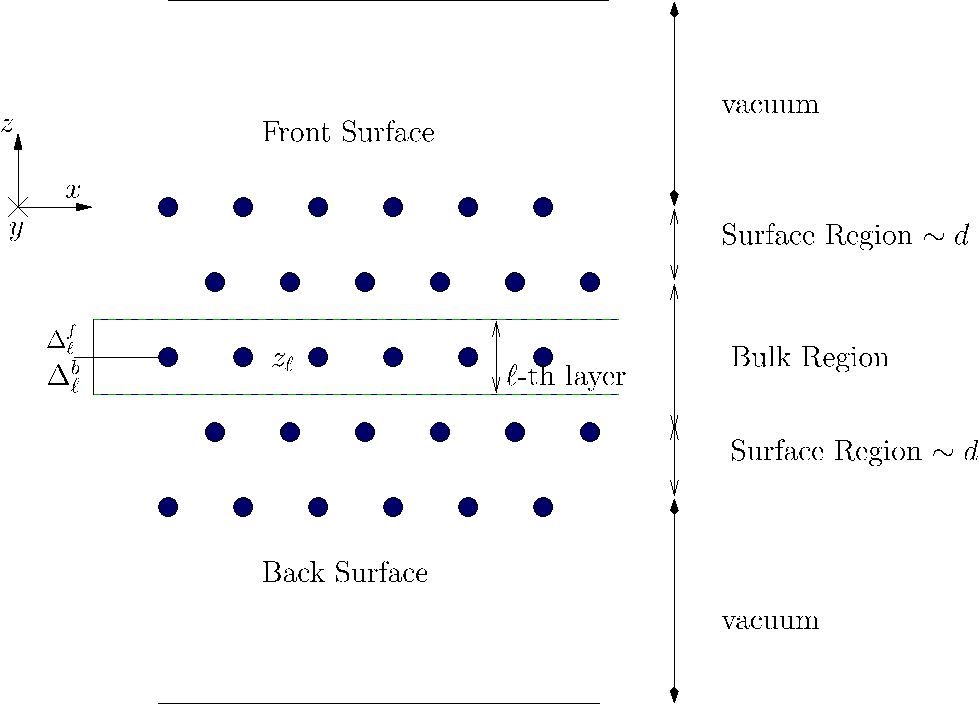
\includegraphics[scale=.7]{images/slab}
\caption{(color on line) A sketch of the super-cell. 
The atomic slab corresponds to the
circles representing the atoms of the system.
\label{fslab}} 
\end{figure}

To introduce the
cut function ${\mathbf{\cal C}}(z)$ in
the calculation of $\chi^{\mathrm{a}\mathrm{b}\mathrm{c}}$, we start from 
the operator for the electron current,
$\mathbf{j}(\mathbf{r})=\frac{e}{2}\left(\mathbf{v}^\Sigma | \mathbf{r}\rangle\langle\mathbf{r} |
+ | \mathbf{r}\rangle\langle\mathbf{r} | \mathbf{v}^\Sigma\right)$, that leads to
\begin{equation}
\mathbf{j}^{(N)}(\mathbf{r},t)=\mathrm{Tr}(\mathbf{j}(\mathbf{r})\rho^{(N)}(t))
=
\int \frac{dk^3}{8\pi^3}
\sum_{nm}
\rho^{(N)}_{nm}(\mathbf{k};t)\mathbf{j}_{mn}(\mathbf{k};\mathbf{r})
,
\label{jmic}
\end{equation}
where 
\begin{equation}
\mathbf{j}_{mn}(\mathbf{k};\mathbf{r})=
\frac{e}{2}
\left(
\langle m\mathbf{k} | \mathbf{v}^\Sigma | \mathbf{r}\rangle \langle\mathbf{r}|n\mathbf{k}\rangle
+
\langle m\mathbf{k}|\mathbf{r}\rangle\langle\mathbf{r} | \mathbf{v}^\Sigma | n\mathbf{k}\rangle
\right).
\label{jmic3}
\end{equation}
Integrating the microscopic current $\mathbf{j}(\mathbf{r},t)$ over
the entire slab gives the averaged microscopic current density, $\mathbf{J}(t)$. 
If we want the contribution from only one region of the unit cell 
towards the total current, we can integrate $\mathbf{j}({\mathbf r},t)$ 
over the desired region. Then the contribution 
to the current density from the
chosen region of the slab is given by
\begin{equation*}
\frac{1}{A}\int d^3r\, {\mathbf{\cal C}}(z)\, 
\mathbf{J}^{(N)} (\mathbf{r},t)
 \equiv \boldsymbol{\mathcal{\cal J}}^{(N)}(t),
\end{equation*}
where $\boldsymbol{\mathcal{\cal J}}^{(N)}(t)$ is the $N$-th order current induced in the
region specified by ${\mathbf{\cal C}}(z)$.
Therefore we define
\begin{equation}
e{\boldsymbol{\mathcal{V}}}^{\Sigma}_{mn}(\mathbf{k})
\equiv
\int d^3r\, {\mathbf{\cal C}}(z)\,\mathbf{j}_{mn}({\mathbf{k}};\mathbf{r}),
\label{vcal}
\end{equation}
to write the Fourier transform of Eq.~\eqref{jmic} as
\begin{equation}
\boldsymbol{\mathcal{\cal J}}^{(N)}(2\omega)=\frac{e}{A}
\int \frac{dk^3}{8\pi^3}
\sum_{mn}
\boldsymbol{\mathcal{\cal V}}^{\Sigma}_{mn}(\mathbf{k}) 
\rho^{(N)}_{nm}(\mathbf{k};2\omega) 
, 
\label{jmac2}
\end{equation}
that gives the induced microscopic current of the chosen region, to order $N$ 
in the external perturbation. 
From
Eqs.~\eqref{vcal} and \eqref{jmic3} we obtain
\begin{align*}
{\boldsymbol{\mathcal{V}}}^{\Sigma}_{mn}({\mathbf k})
&=
\frac{1}{2}
\int \mathrm{d}^3 r\,
 {\mathbf{\cal C}}(z)
\bigg[
\langle m\mathbf{k}|\mathbf{v}^\Sigma | \mathbf{r}\rangle
\langle \mathbf{r} | n \mathbf k \rangle +
\langle m\mathbf{k} | \mathbf{r}\rangle
\langle \mathbf{r} | \mathbf{v}^\Sigma | n \mathbf k \rangle\bigg]
\nonumber\\
&=
\frac{1}{2}
\int \mathrm{d}^3 r\,
 {\mathbf{\cal C}}(z)
 \bigg[
\psi_{n\mathbf{k}}(\mathbf{r})
\mathbf{v}^{\Sigma *}\psi^*_{m\mathbf{k}}(\mathbf{r})
+ 
\psi^*_{m\mathbf{k}}(\mathbf{r})\mathbf{v}^\Sigma
\psi_{n\mathbf{k}}(\mathbf{r})
\bigg]
\nonumber\\
&=
\int \mathrm{d}^3 r\,
\psi^*_{m\mathbf{k}}(\mathbf{r})
\left[\frac{{\mathbf{\cal C}}(z) \mathbf{v}^\Sigma +
\mathbf{v}^\Sigma {\mathbf{\cal C}}(z)}{2}\right]
\psi_{n\mathbf{k}}(\mathbf{r})
\nonumber\\
&=
\int \mathrm{d}^3 r\,
\psi^*_{m\mathbf{k}}(\mathbf{r})
\boldsymbol{\mathcal{\cal V}}^{\Sigma}
\psi_{n\mathbf{k}}(\mathbf{r})
,
\end{align*}
where, we used the hermitian property of $\mathbf{v}^\Sigma$ and defined
\begin{equation*}
\boldsymbol{\mathcal{\cal V}}^{\Sigma}
=
\frac{{\mathbf{\cal C}}(z) \mathbf{v}^\Sigma +
\mathbf{v}^\Sigma {\mathbf{\cal C}}(z)}{2}
.
\end{equation*} 
We see that the replacement
\begin{equation}
\mathbf{V} \to \boldsymbol{\mathcal{\cal V}}=\frac{{\mathbf{\cal C}}(z) \mathbf{V} +
\mathbf{V} {\mathbf{\cal C}}(z)}{2}
,
\label{vcali}
\end{equation} 
is all that is needed to change any of the
electron velocity operators $\mathbf{V}$ to the new velocity
operator $\boldsymbol{\mathcal{\cal V}}$ that implicitly takes into account the
contribution of the region of the slab given by ${\mathbf{\cal C}}(z)$.
We note that this modified operator is hermitian as it should.\cite{note2}
The operator $\mathbf{V}$ could be any of those given by Eq.~\eqref{vop2},
thus
\begin{align*}
\boldsymbol{\mathcal{\cal V}}^{\Sigma}
&=
\boldsymbol{\mathcal{\cal V}}^{\mathrm{LDA}}
+
\boldsymbol{\mathcal{\cal V}}^{S}
\nonumber\\
\boldsymbol{\mathcal{\cal V}}^{\mathrm{LDA}}
&=
\boldsymbol{\mathcal{\cal V}}
+
\boldsymbol{\mathcal{\cal V}}^{\mathrm{nl}}
.
\end{align*}
To calculate
$\boldsymbol{\mathcal{\cal V}}^{\Sigma}_{nm}(\mathbf{k})$ 
we calculate the matrix elements of 
$\boldsymbol{\mathcal{\cal V}}^{\mathrm{LDA}}$ and $\boldsymbol{\mathcal{\cal V}}^{S}$
 (separately)
according to the expressions of
Appendices \ref{calpcalc} and \ref{calvs}.
If not stated differently, calligraphic letters correspond to layer quantities. 

To limit the SHG response to one surface, Eq.~\eqref{vcali} 
for $\boldsymbol{\mathcal{\cal V}}$ was proposed in 
Ref.~\onlinecite{reiningPRB94} and later used in Refs.
\onlinecite{mendozaPRL98},
\onlinecite{mendozaPRB01},
\onlinecite{sanoPRB02},
 and \onlinecite{mejiaRMF04}. 
In this article, for the first time, we formally introduce the cut function ${\mathbf{\cal C}}(z)$ 
for the second-harmonic optical response of semiconductor surfaces,
from an average of the second order polarization over the region of interest.

Using
$\boldsymbol{\mathcal{\cal J}}=d\boldsymbol{\mathcal{\cal P}}/dt$ 
and Eq.~\eqref{jmac2} 
we obtain the SH polarization of a given region as
\begin{equation}
\boldsymbol{\mathcal{\cal P}}^{(2)}(2\omega)
=\frac{ie}{2A\tilde\omega}
\int \frac{dk^3}{8\pi^3}
\sum_{mn}
\boldsymbol{\mathcal{\cal V}}^{\Sigma}_{mn}(\mathbf{k})
\rho^{(2)}_{nm}(\mathbf{k};2\omega)
,
\label{Pjikn}
\end{equation}
and using Eqs.~\eqref{pshg} and \eqref{j.2} 
leads to
\begin{align}
\chi^{\mathrm{a}\mathrm{b}\mathrm{c}}(-2\omega;\omega,\omega) 
&=
\frac{e^2}{2A\hbar\tilde\omega}
\int \frac{dk^3}{8\pi^3}
\sum_{mn}
\frac{{\mathbf{\cal V}}^{\Sigma,\mathrm{a}}_{mn}(\mathbf{k})}
{\omega^\Sigma_{nm\mathbf{k}}-2\tilde\omega}
\bigg[
-(B_{nm}^{\mathrm{c}}(\mathbf{k},\omega))_{;k^{\mathrm{b}}}
\nonumber \\
&
+i\sum_q\left(r_{nq}^{\mathrm{b}}B_{qm}^{\mathrm{c}}(\mathbf{k},\omega) -
  B_{nq}^{\mathrm{c}}(\mathbf{k},\omega) 
  r_{qm}^{\mathrm{b}}\right)
\bigg]
,
\label{Pjikn2}
\end{align}
which gives the susceptibility 
$\chi^{\mathrm{a}\mathrm{b}\mathrm{c}}(-2\omega;\omega,\omega)$ 
of the layers of the slab specified by ${\mathbf{\cal C}}(z)$. 
We mention that the units of 
$\chi^{\mathrm{a}\mathrm{b}\mathrm{c}}(-2\omega;\omega,\omega)$
are m$^2$/V, as they should be for a surface SH susceptibility.
Using Eq.~\eqref{j.1} we
split this equation into
two contributions from the first and second terms on the right hand side
of Eq.~\eqref{Pjikn2}:
\begin{equation}
\chi^{\mathrm{a}\mathrm{b}\mathrm{c}}_i (-2\omega;\omega,\omega)
=-\frac{e^3}{A\hbar^22\tilde\omega}
\int \frac{dk^3}{8\pi^3}
\sum_{mn}
\frac{{\mathbf{\cal V}}_{mn}^{\Sigma,\mathrm{a}}}{\omega^\Sigma_{nm}-2\tilde\omega}
\left(\frac{f_{mn}r_{nm}^{\mathrm{b}}}{\omega^\Sigma_{nm}-\tilde\omega}\right)_{;k^{\mathrm{c}}}
,
\label{chii}
\end{equation} 
related to intraband transitions, and 
\begin{equation}
\chi^{\mathrm{a}\mathrm{b}\mathrm{c}}_e (-2\omega;\omega,\omega)
=\frac{ie^3}{A\hbar^22\tilde\omega}
\int \frac{dk^3}{8\pi^3}
\sum_{qmn}
\frac{{\mathbf{\cal V}}_{mn}^{\Sigma,\mathrm{a}}}{\omega^\Sigma_{nm}-2\tilde\omega}
\left(
\frac{r_{nq}^{\mathrm{c}} r_{qm}^{\mathrm{b}} 
f_{mq}}{\omega^\Sigma_{qm}-\tilde\omega}
-\frac{r_{nq}^{\mathrm{b}} r_{qm}^{\mathrm{c}} 
f_{qn}}{\omega^\Sigma_{nq}-\tilde\omega}
\right),
\label{chie}
\end{equation} 
related to interband transitions.
The generalized derivative in Eq.~\eqref{chii} is dealt with by the chain rule 
\begin{equation}
\left(\frac{f_{mn}r_{nm}^{\mathrm{b}}}{\omega^\Sigma_{nm}-\tilde\omega}\right)_{;k^{\mathrm{c}}}=
\frac{f_{mn}}{\omega^\Sigma_{nm}-\tilde\omega}\left(r_{nm}^\mathrm{b}\right)_{;k^{\mathrm{c}}}
-\frac{f_{mn}r_{nm}^{\mathrm{b}}\Delta_{nm}^\mathrm{c}}{(\omega^\Sigma_{nm}-\tilde\omega)^2}
,
\label{gene2}
\end{equation}
where substituting $H^\Sigma_0$ 
into Eq.~\eqref{conmri3n} and then
Eq.~\eqref{chon.10}
we obtain
\begin{equation*}
\left(\omega^\Sigma_{nm}\right)_{;k^{\mathrm{a}}}
=
\left(\omega^\mathrm{LDA}_{nm}\right)_{;k^{\mathrm{a}}}
= 
v_{nn}^{\mathrm{LDA},\mathrm{a}}-v_{mm}^{\mathrm{LDA},\mathrm{a}}\equiv\Delta_{nm}^{\mathrm{a}}
.
\end{equation*} 
The apparent divergence as $\tilde\omega\to 0$
in Eqs. \eqref{chii} and \eqref{chie},  
is removed  by
 a partial fraction expansion over $\tilde\omega$. 
Using time-reversal symmetry, an integration by parts to 
remove the square in the denominator of the second term of Eq.~\eqref{gene2}, 
and taking the limit of $\eta\to 0$, 
we obtain the following expressions for the imaginary parts of 
Eqs. \eqref{chii} and \eqref{chie}, 
\begin{subequations}\label{chis}
\begin{equation}
\mathrm{Im}[\chi^{\mathrm{a}\mathrm{b}\mathrm{c}}_{e,\omega}]= 
\frac{\pi |e|^3}{2\hbar^2}
\int \frac{dk^3}{8\pi^3}
\sum_{vc}\sum_{q\neq(v,c)}\frac{1}{\omega^\Sigma_{cv}}
\left[
\frac{\mathrm{Im}[\mathcal{V}^{\Sigma,\mathrm{a}}_{qc}\{r^{\mathrm{b}}_{cv}r^{\mathrm{c}}_{vq}\}]}
{(2\omega^\Sigma_{cv}-\omega^\Sigma_{cq})} 
-\frac{\mathrm{Im}[\mathcal{V}^{\Sigma,\mathrm{a}}_{vq}\{r^{\mathrm{c}}_{qc}r^{\mathrm{b}}_{cv}\}]}
{(2\omega^\Sigma_{cv}-\omega^\Sigma_{qv})}
\right]\delta(\omega^\Sigma_{cv}-\omega),
\end{equation}  
\begin{equation}
\mathrm{Im}[\chi^{\mathrm{a}\mathrm{b}\mathrm{c}}_{i,\omega}]= 
\frac{\pi\vert e\vert^3}{2\hbar^2}
\int \frac{dk^3}{8\pi^3}
\sum_{cv}\frac{1}{(\omega^\Sigma_{cv})^{2}}
\left[
\mathrm{Re}\left[\left\{r^{\mathrm{b}}_{cv}\left(\mathcal{V}^{\Sigma,\mathrm{a}}_{vc}\right)_{;k^{\mathrm{c}}}\right\}\right]
+\frac{\mathrm{Re}\left[\mathcal{V}^{\Sigma,\mathrm{a}}_{vc}\left\{r^{\mathrm{b}}_{cv}
\Delta^{\mathrm{c}}_{cv}\right\}\right]}{\omega^\Sigma_{cv}} 
\right]\delta(\omega^\Sigma_{cv}-\omega),
\end{equation}
\begin{equation}
\mathrm{Im}[\chi^{\mathrm{a}\mathrm{b}\mathrm{c}}_{e,2\omega}]= 
-\frac{\pi |e|^3}{2\hbar^2}
\int \frac{dk^3}{8\pi^3}
\sum_{vc}\frac{4}{\omega^\Sigma_{cv}}
\left[
\sum_{v'\ne
  v}\frac{\mathrm{Im}[\mathcal{V}^{\Sigma,\mathrm{a}}_{vc}\{r^{\mathrm{b}}_{cv'}r^{\mathrm{c}}_{v'v}\}]}
{2\omega^\Sigma_{cv'}-\omega^\Sigma_{cv}}
- \sum_{c'\ne
  c}\frac{\mathrm{Im}[\mathcal{V}^{\Sigma,\mathrm{a}}_{vc}\{r^{\mathrm{c}}_{cc'}r^{\mathrm{b}}_{c'v}\}]}
{2\omega^\Sigma_{c'v}-\omega^\Sigma_{cv}}
\right]\delta(\omega^\Sigma_{cv}-2\omega),
\end{equation}
\begin{equation}
\mathrm{Im}[\chi^{\mathrm{a}\mathrm{b}\mathrm{c}}_{i,2\omega}]= 
 \frac{\pi \vert
   e\vert^{3}}{2\hbar^2}
\int \frac{dk^3}{8\pi^3}
\sum_{vc}\frac{4}{(\omega^\Sigma_{cv})^{2}}
\left[\mathrm{Re}\left[\mathcal{V}^{\Sigma,\mathrm{a}}_{vc}\left\{\left(r^{\mathrm{b}}_{cv}\right)_{;k^{\mathrm{c}}}
\right\}\right] -
\frac{2\mathrm{Re}\left[\mathcal{V}^{\Sigma,\mathrm{a}}_{vc}\left\{r^{\mathrm{b}}_{cv}
\Delta^{\mathrm{c}}_{cv}\right\}\right]}{\omega^\Sigma_{cv}}\right]\delta(\omega^\Sigma_{cv}-2\omega)
,
\end{equation}
\end{subequations}
where we have split the interband and intraband $1\omega$ and $2\omega$
contributions and supressed the $\omega$ arguments for 
convenience of notation.
The factor of 2 for spin degeneracy is not included in Eq.~\eqref{chis}. 
The real part of each contribution can be obtained through
a Kramers-Kronig transformation\cite{nicolasPRB14} and
$\chi^{\mathrm{a}\mathrm{b}\mathrm{c}}=
\chi^{\mathrm{a}\mathrm{b}\mathrm{c}}_{e,\omega} 
+\chi^{\mathrm{a}\mathrm{b}\mathrm{c}}_{e,2\omega}
+\chi^{\mathrm{a}\mathrm{b}\mathrm{c}}_{i,\omega} 
+\chi^{\mathrm{a}\mathrm{b}\mathrm{c}}_{i,2\omega}
$.
To fulfill the required intrinsic permutation symmetry, 
the $\{\}$ notation symmetrizes the $\mathrm{b}\mathrm{c}$ Cartesian indices, i.e. 
$\{u^{\mathrm{b}}s^{\mathrm{c}}\}=(u^{\mathrm{b}}s^{\mathrm{c}}+u^{\mathrm{c}}s^{\mathrm{b}})/2$,
and thus
$\chi^{\mathrm{a}\mathrm{b}\mathrm{c}}=\chi^{\mathrm{a}\mathrm{c}\mathrm{b}}$.
The full expressions for
$\chi^{\mathrm{a}\mathrm{b}\mathrm{c}}(-2\omega;\omega,\omega)$, along 
with the various quantities involved in Eq.~\eqref{chis} are given in
the Appendix \ref{appe}. 
We mention that if we take ${\mathbf{\cal C}}(z)=1$ through out, the layered
matrix elements $\boldsymbol{\mathcal{\cal V}}^{\Sigma}_{nm}$ become standard bulk-like
$\mathbf{v}^{\Sigma}_{nm}$ matrix elements. We mention that in this
case, Eq.~\eqref{chis} is equivalent to the expressions of
Ref.~\onlinecite{cabellosPRB09}, valid for bulk semiconductors.
 
Finally, we could also calculate the nonlinear surface susceptibility as 
\begin{equation}
\boldsymbol{\chi}(-2\omega;\omega,\omega)
= \sum_{\{\ell\}}\boldsymbol{\chi}^\ell(-2\omega;\omega,\omega),
\label{chiijksur}
\end{equation} 
where $\ell$ would denote a particular layer chosen through
${\mathbf{\cal C}}^\ell(z)$ of Eq.~\eqref{sz} and
$\{\ell\}$
is meant to be a chosen set of layers. For instance, 
one can take a single layer 
encompassing half of the slab, or take each 
atomic layer individually to the middle
of the slab. For the first case there is 
a single summand
in Eq.~\eqref{chiijksur}. For the second case
there is a sum from $\ell=1$, denoting the first layer 
right at the surface, to $\ell=N$, denoting the layer at the middle of the slab 
that behaves like a bulk layer.
We remark that the value of 
$N$ is not universal and
the slab needs to have enough atomic layers 
in order to give converged results for 
$\boldsymbol{\chi} (-2\omega;\omega,\omega)$. 
We can use Eq.~\eqref{chiijksur} for 
either the front or the back surface. 

\section{Results}\label{results}

In this section we present a 
relevant test case to check the
consistency of our approach. We have selected
a clean Si(001) surface with a $2\times 1$ surface reconstruction.
The slab for such a surface could be chosen to be centrosymmetric 
by creating the front and back
surfaces with the same $2\times 1$
reconstruction. However, we choose to terminate one 
of the surfaces with hydrogen producing an ideal  
terminated bulk Si surface. The H atoms simply saturate the 
dangling bonds of the bulk-like Si atoms at the surface, as seen in 
Fig.~\ref{si2x1}.
We take the $z$ coordinate pointing out of the surface and the $x$
coordinate along the crystallographic [011] direction is parallel to the dimmers. 
\begin{figure}
\centering 
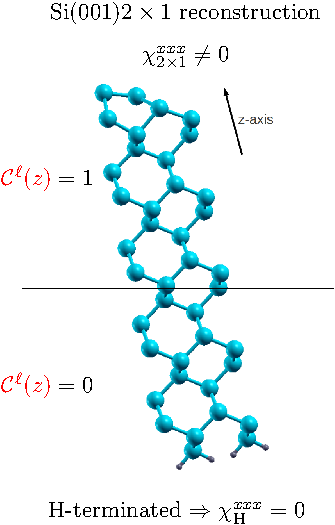
\includegraphics[scale=.8]{images/si2x1-crop}
\caption{(color on line) The slab shows a 
    clean Si(001)$2\times 1$ front surface 
    with an ideal terminated Si bulk back surface. The
    dangling bonds are H (small balls) saturated. 
    This image depicts 12 Si atomic layers
    with one H atomic layer. 
\label{si2x1}} 
\end{figure} 
The idea behind this slab configuration is that the 
cristalline symmetry of the H terminated surface imposes that 
$\chi_{\mathrm{H}}^{xxx}=0$.
 The $2\times 1$ surface has no 
such restrictions, so $\chi_{2\times 1}^{xxx}\ne 0$.
This is due to the fact that along the $y$ direction there is a mirror plane for the
H-saturated surface, whereas 
for the $2\times 1$ surface this mirror is lost as the dimers are
asymmetric along $x$. 
Thus, calculating $\chi^{xxx}$ for the full-slab, or the 
half-slab containing the $2\times 1$ surface\cite{note1}
should yield the same result since the contribution from the H
saturated surface is zero regardless. 
We must check that the following 
relationship is satisfied for this particular slab
\begin{equation*}
\chi_{\mathrm{half-slab}}^{xxx}(-2\omega;\omega,\omega) 
=
\chi_{\mathrm{full-slab}}^{xxx}(-2\omega;\omega,\omega) 
,
\end{equation*}
where
$\chi_{\mathrm{half-slab}}^{xxx}(-2\omega;\omega,\omega)$ is calculated using
${\mathbf{\cal C}}(z)=1$ from the upper half containing the $2\times 1$ 
surface reconstruction, as seen in Fig.~\ref{si2x1},
and $\chi_{\mathrm{full-slab}}^{xxx}(-2\omega;\omega,\omega)$ is calculated using
${\mathbf{\cal C}}(z)=1$ through the full slab.
We show the results for this comparison in the remainder  
of this section.  
Also, we checked that 
for the
dihydride surface
$\chi_{\mathrm{half-slab}}^{xxx}(-2\omega;\omega,\omega)=0$.

The self-consistent ground state and the Kohn-Sham states were
calculated in the DFT-LDA framework using the plane-wave 
ABINIT code.\cite{abinit}
We used Troullier-Martins pseudopotentials\cite{troullierPRB91} that are 
fully separable nonlocal pseudopotentials in the Kleinman-Bylander 
form.\cite{kleinmanPRL82}
The contribution of $\mathbf{v}^\mathrm{nl}$ 
and 
$\boldsymbol{\mathcal{\cal V}}^\mathrm{nl}$ 
to Eq.~\eqref{chis} is carried out 
using the DP code.\cite{olevanoDP}
The surfaces have been studied with the experimental lattice constant of 5.43 \AA. 
Structural optimizations were performed 
with the ABINIT code.\cite{abinit}  
The geometry optimization has been carried out in slabs of 12
atomic layers where the central four layers where fixed at the bulk
positions.  
The structures were relaxed until the Cartesian force components were less than 5 meV/\AA. 
The geometry optimization for the clean surface gives
a dimer buckling of 0.721 \AA, and a dimer length of 2.301 \AA.  
For the  Si(001)$1\times 1$:2H dihydride surface, we have obtained a Si-H bond distance of 1.48 \AA. 
This results are in good agreement with previous 
theoretical studies.\cite{caramellaPRB09,mendozaPRB06}
The vacuum size is equivalent to one quarter the
size of the slab, avoiding the effects produced by possible 
wave-function tunneling from the contiguous surfaces of the full
crystal formed by the repeated super-cell scheme.\cite{mendozaPRB06}    

Spin-orbit, local field, and electron-hole 
attraction\cite{beyond}
effects on the SHG process are all neglected.
Although these are important factors in the optical response of a semiconductor,
their efficient calculation is still theoretically and  
numerically challenging and  
under debate. This merits further study but is beyond the scope of this paper.
For a given slab size, we find the converged spectra 
to obtain the relevant parameters. The most important of 
these are: an energy cut-off of 10 Ha for the 16, 24, and 32 layered
slabs
and 13 Ha for the 40 layer slab,
an equal number of conduction and 
valence bands, and a set of 244 $\mathbf{k}$-points.
The $\mathbf{k}$-points are used for the linear analytic 
tetrahedron method for evaluating the
Brillouin zone integrals 
where special care was taken to examine the double resonances
of Eq.~\eqref{chis}. \cite{nastosPRB05}
All spectra were calculated with a Gaussian smearing of 0.15 eV.
\begin{figure}
\centering 
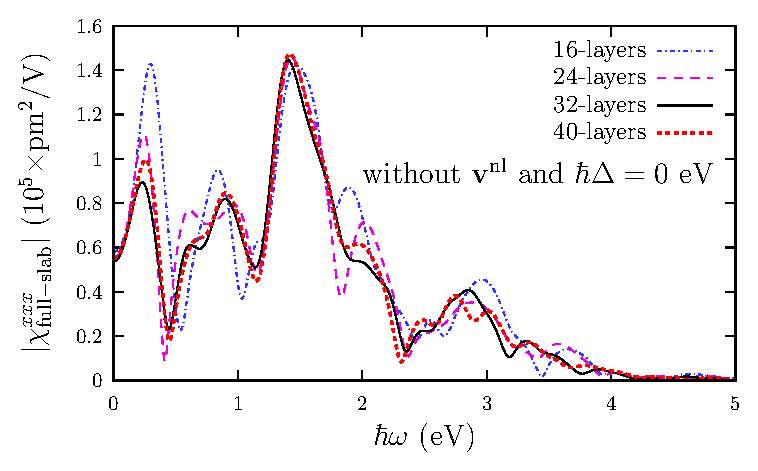
\includegraphics[scale=.8]{plots/fig1}
\caption{(color on line) 
$|\chi_{\mathrm{half-slab}}^{xxx}|$ vs $\hbar\omega$ 
for the slab
with 16, 24, 32, and 40 atomic Si layers. The front surface 
is in a clean $2\times 1$ reconstruction and the back 
surface is an ideal terminated bulk H-saturated dangling bonds (see Fig.~\ref{si2x1}).
\label{fig1}} 
\end{figure}
\begin{figure}
\centering 
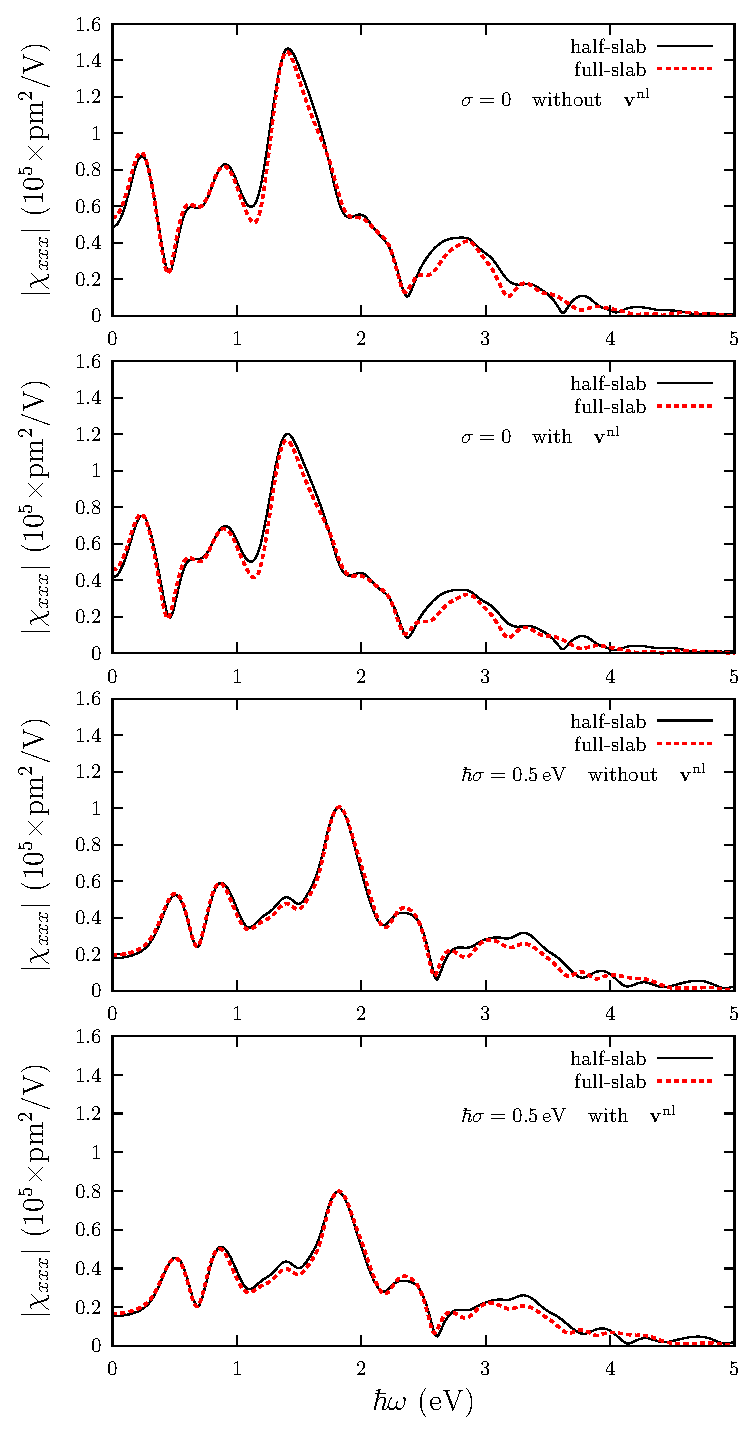
\includegraphics[scale=.8]{plots/fig2}
\caption{(color on line) 
$\chi^{xxx}_{\mathrm{half-slab}}$
and 
$\chi^{xxx}_{\mathrm{full-slab}}$
vs $\hbar\omega$ for a slab with 32 
atomic Si layers plus one H layer. 
\label{fig2}} 
\end{figure}

We must evaluate 
$T^{\mathrm{a}\mathrm{b}}_{nm}=(i/\hbar)[r^\mathrm{b},v^{\mathrm{nl},\mathrm{a}}]_{nm}$
in order to obtain 
Eqs.~\eqref{tau.1} and \eqref{tau.1n} that are required for 
Eq.~\eqref{chis}.
Computing second-order 
derivatives is required thus making the numerical procedure very 
time consuming. This adds significantly to the already lengthy time needed 
for the calculation of the $\mathbf{v}^\mathrm{nl}$ contribution that is
proportional only to 
the first order derivatives. 
Memory requirements are also increased for both $\mathbf{v}^\mathrm{nl}$ and 
$[\mathbf{r},\mathbf{v}^\mathrm{nl}]$. However, the contribution from $[\mathbf{r},\mathbf{v}^\mathrm{nl}]$ 
is very small\cite{valerie} and therefore we neglect it in this work.

\subsection{Full-slab results}\label{fsresults}

In Fig.~\ref{fig1} we show $|\chi_{\mathrm{full-slab}}^{xxx}|$
for the slab with
16, 24, 32, and 40 Si atomic layers, without the contribution of
$\mathbf{v}^{\mathrm{nl}}$ and with no scissors correction.
Since the clean Si(001) surface is $2\times 1$,
there are two atoms per atomic layer, thus the total number of atoms per slab is 
twice the number of atomic layers of the slab. 
In making the slabs larger, we add steps of 8 layers of bulk-like atomic positions. 
We note that the response differs substantially 
for 16 and 24 layers but is quite similar for 32 and 40 layers.
As explained above,
the calculation of the $\mathbf{v}^\mathrm{nl}$ contribution is 
computationally expensive.
A good compromise between the accuracy in the convergence of
$\chi^{xxx}_{\mathrm{full-slab}}$ as a function of the number
of layers in the slab, and the computational 
expense is to consider
the slab with 32 Si atomic layers as 
an accurate representation of our 
system.

\subsection{Half-slab vs. full-slab}

In Fig.~\ref{fig2}
we compare 
$\chi^{xxx}_{\mathrm{half-slab}}$  
vs. 
$\chi^{xxx}_{\mathrm{full-slab}}$ 
for the four different possibilities 
between including or not including the
effects of $\mathbf{v}^\mathrm{nl}$ or the scissors correction
$\hbar\Delta$.   
For these results we chose
$\hbar\Delta=0.5$ eV, that is the GW gap reported in
Refs.~\onlinecite{rohlfingPRB95,garciaCPC01}. 
{\color{\chon}This is justified by the fact that the surface states of the clean 
Si(001) surface investigated are found, from GW calculations 
\cite{rohlfingPRB95}, to shift rigidly and to keep their dispersion with 
respect to LDA.}
We see that for all four instances the 
difference between responses is quite small.
Indeed, when the value $|\chi^{xxx}|$ 
is large the difference between the two is very small; 
when the value is small the difference increases only slightly, 
but the spectra is so close to zero that it is negligible. 
These differences would decrease as the number of atomic layers 
increases. We remark that 32 layers in the slab is more than enough 
to confirm that the extraction of the surface second-harmonic 
susceptibility from the $2\times 1$ surface is readily possible 
using the formalism contained in Eq.~\eqref{chis}.
We have confirmed that for the dihydride surface
$|\chi^{xxx}_{\mathrm{half-slab}}|\approx 0$ (not shown).
This confirms the validity of our theory and is the main result of
this article; through the proposed layer formalism we can calculate the surface SH
$\chi^{\mathrm{a}\mathrm{b}\mathrm{c}}(-2\omega;\omega,\omega)$    
including
the
contribution of the nonlocal part of the pseudopotentials 
and the part of the many-body effects through the scissors correction.
Our scheme should work for any slab.

\subsection{\texorpdfstring{Results for $\chi^{xxx}_{2\times 1}(-2\omega;\omega,\omega)$}
{Results for Xxxx(2x1)(-2w;w,w)}}

We proceed to explain 
some of the features seen in $|\chi^{xxx}_{2\times 1}|$ that, as
explained above, are obtained 
by calculating $|\chi^{xxx}_{\mathrm{half-slab}}|$.
First, from Fig.~\ref{fig2} we note a series of resonances 
that derive from 1$\omega$ and 2$\omega$ terms in
Eq.~\eqref{chis}. 
Notice that the 
2$\omega$ resonances start below $E_g/2$ where $E_g$ is the band gap
(0.53 eV  for LDA and
1.03 eV if the scissor is used with
$\hbar\Delta=0.5$ eV).
These resonances
come from the electronic states of the 
$2\times 1$ surface, that lie inside the bulk band gap of Si and are the 
well known electronic surface states.\cite{rohlfingPRB95} 
In Fig.~\ref{fig3}
we see that the effect of $\mathbf{v}^\mathrm{nl}$
 reduces the value of   
$|\chi^{xxx}_{2\times 1}|$  
by 15-20\% 
showing the importance of this contribution for a correct calculation  
of SSHG, in agreement with the analysis for bulk semiconductors.\cite{luppiPRB08}
However, the inclusion of $\mathbf{v}^\mathrm{nl}$ does not
changes the 
spectral shape of $|\chi^{xxx}_{2\times 1}|$;
 this also can be confirmed from
the cases of zero scissors correction from Fig.~\ref{fig2}.
\begin{figure}
\centering 
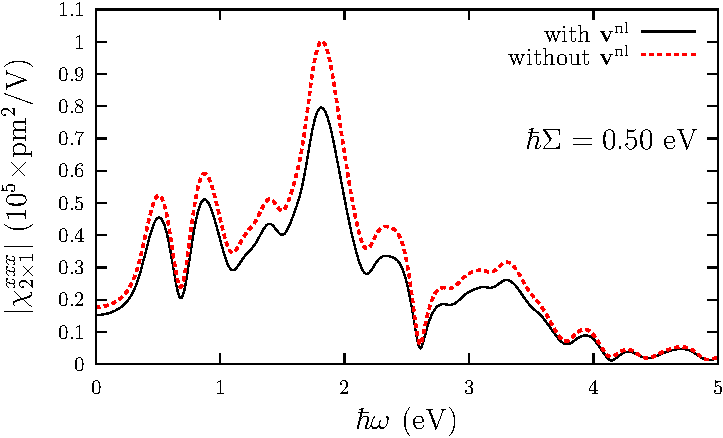
\includegraphics[scale=.8]{plots/fig3}
\caption{(color on line) 
$\chi^{xxx}_{2\times 1}$
vs $\hbar\omega$ for a slab with 32 
atomic Si layers plus one H layer, 
with and without the contribution from $\mathbf{v}^\mathrm{nl}$.
\label{fig3}} 
\end{figure}

To see the effect of the scissors correction, we take two different
finite values for $\hbar\Delta$. The first one
with a value of $\hbar\Delta=0.5$ eV, used in the above results, 
is the ``average'' GW gap taken from 
Ref.~\onlinecite{rohlfingPRB95} 
that is in agreement with Ref.~\onlinecite{garciaCPC01}. The second one
with a value of $\hbar\Delta=0.63$ eV is the ``average'' 
gap taken from Ref.~\onlinecite{asahiPRB00}, 
where more $\mathbf{k}$-points in the Brillouin zone were 
used to calculate its GW value.
From Fig.~\ref{fig4}
we note that the scissors correction 
shifts the spectra from it LDA value to higher energies as expected.
 However, contrary 
to the case of linear optics\cite{cabellosPRB09} the shift introduced 
by the scissors correction is not 
rigid, as pointed out in Ref.~\onlinecite{nastosPRB05}. 
 This is because the second-harmonic optical response mixes 
$1\omega$ and $2\omega$ transitions (see Eq.~\eqref{chis}), and accounts 
for the non-rigid shift. {\color{\chon}The reduction of the spectral strength is in 
agreement with previous calculations for bulk systems.
\cite{nastosPRB05, luppiPRB10, leitsmannPRB05}}
When we compare 
$|\chi^{xxx}_{2\times 1}|$ for the two finite values of $\hbar\Delta$,
we see that the first two peaks are almost rigidly 
shifted with a small difference in height while
the rest of the peaks are modified substantially. 
This behavior comes from the fact that the first two
peaks are almost exclusively related to the 
2$\omega$ resonances of
Eq.~\eqref{chis}. The other peaks are a combination 
of 1$\omega$ and 2$\omega$ resonances 
and yield a more varied spectrum.
We mention that for large gap materials, the 1$\omega$ and 2$\omega$ would be splited
showing a small interference effect, but still the 2$\omega$ would
strongly depend on the surface states.
 This way we see that small changes in the value of the 
scissors shift can in general affect the SSH susceptibility 
spectrum quite dramatically.
In Ref.~\onlinecite{adolphPRB00}, the authors already remarked
that nonlinear optical response of bulk materials
is more influenced by the electronic structure
of the material than the linear case. 
In the case of semiconducting surfaces the
problem is even more intricate due to the presence of electronic
surface states.
The high sensitivity of SSHG to the energy position  of surface
states, as seen in Fig.~\ref{fig4}, makes SSHG a good benchmark
spectroscopical tool for testing the validity of the inclusion of many-body effects,
and in particular the quasi-particle correction to the electronic states. 
\begin{figure}
\centering 
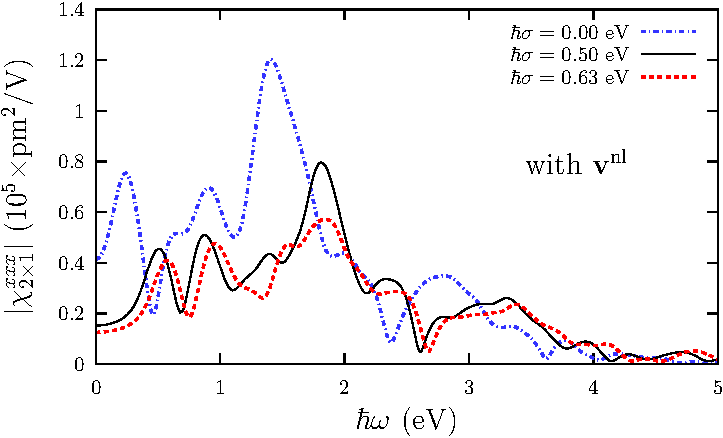
\includegraphics[scale=.8]{plots/fig4}
\caption{(color on line) 
$\chi^{xxx}_{2\times 1}$
vs $\hbar\omega$ for a slab with 32 
atomic Si layers plus one H layer, 
for two different values of 
the scissors correction $\hbar\Delta$. 
\label{fig4}} 
\end{figure}

Although local fields are neglected they should, in principle, 
be small parallel to the interface as the electric field is continuous.
So, we would expect that the $xxx$ component of 
$\boldsymbol{\chi}(-2\omega;\omega,\omega)$ 
would have a small influence from the local fields.
Also, the excitonic effects ought to be explored, but
their efficient calculation is theoretically and 
numerically challenging\cite{beyond}   and beyond the scope 
of this article.
Unfortunately the experimental measurement of the $xxx$
component of $\boldsymbol{\chi}(-2\omega;\omega,\omega)$ is not possible as the SH 
radiated intensity would be proportional not only to this component 
but also to the other components of $\boldsymbol{\chi}(-2\omega;\omega,\omega)$.  
However,
in a forthcoming publication 
we will present a study of SSHG from several 
Si surfaces 
with comparison to experimental 
results. 

\section{Conclusions}\label{conc}

We have presented a formulation to calculate the surface second-harmonic
(SSH) susceptibility tensor $\boldsymbol{\chi}(-2\omega;\omega,\omega)$, using the length gauge
formalism and within the independent particle approximation (IPA).
It includes on equal footing:
(i) the scissors correction, 
(ii) the  
contribution of the non-local part of the pseudopotentials, and  
(iii) the cut function.
We have used a Si(001)$2\times 1$ surface to confirm that our scheme
correctly obtains the surface response as we confirm
that 
$\chi_{\mathrm{half-slab}}^{xxx}(-2\omega;\omega,\omega) 
\approx
\chi_{\mathrm{full-slab}}^{xxx}(-2\omega;\omega,\omega) 
. 
$
Although one can in principle increase the number of atomic layers,
$\mathbf{k}$-points, etc. to
improve even further on the similarity of the half-slab and full-slab results, we
have chosen a good compromise between accuracy and the burden and time
of the computations. 
We describe the effect of the independent inclusion of the three
effects mentioned above in the calculation of  
$\boldsymbol{\chi}(-2\omega;\omega,\omega)$. 
The scissors correction shifts the spectrum to  
higher energies though the shifting is not rigid and mixes the 
$1\omega$ and $2\omega$ resonances,  
and has a strong influence in the line-shape,
as for the case of bulk semiconductors.\cite{luppiJCP10,luppiPRB10,leitsmannPRB05}
 The cut function allows us  
to extract unequivocally $\chi^{xxx}_{2\times 1}(-2\omega;\omega,\omega)$.
 The effects of the nonlocal part of the pseudopotentials  
keeps the same line-shape of $|\chi^{xxx}_{2\times
  1}(-2\omega;\omega,\omega)|$,
but  
reduces the value of   
by 15-20\%. 
The $xxx$ component of  
$\boldsymbol{\chi}_{2\times 1}(-2\omega;\omega,\omega)$, 
can not be
experimentally isolated,
however in a forthcoming publication 
we will compare our formulation 
against
experimental 
results. 
We have neglected
local field 
and excitonic effects.
Although these are important factors in the optical response of a semiconductor, 
their efficient calculation is theoretically and  
numerically challenging and still  
under debate.\cite{beyond}   
This merits further study but is beyond the scope of this paper. 
Nevertheless, the inclusion of aforementioned contributions 
in
our scheme opens the unprecedented possibility to study 
surface SHG with more versatility
and 
more accurate results.

\section{Acknowledgments}


B.S.M. acknowledges the Laboratoire des Solides Irradi\'es (Ecole
Polytechnique, Palaiseau, France) for the support and hospitality
during a sabbatical year. B.S.M. acknowledges partial support from
CONACYT-M\'exico Grant 153930. 

%%%%%%%%%%%%%
\appendix 
\section{}\label{appe}
We give explicit expressions for the quantities used in the evaluation 
of Eq.~\eqref{chis}; when appropriate, some 
intermediate steps are given for their derivation. 
\subsection{ Expressions for 
\texorpdfstring{$\chi^{\mathrm{a}\mathrm{b}\mathrm{c}}(-2\omega;\omega,\omega)$}{que} 
}\label{fullchis}
Omitting the frequency dependence for convenience of notation,
$\chi^{\mathrm{a}\mathrm{b}\mathrm{c}}
=
\chi^{\mathrm{a}\mathrm{b}\mathrm{c}}_{e,\omega}
+
\chi^{\mathrm{a}\mathrm{b}\mathrm{c}}_{i,\omega}
+
\chi^{\mathrm{a}\mathrm{b}\mathrm{c}}_{e,2\omega}
+
\chi^{\mathrm{a}\mathrm{b}\mathrm{c}}_{i,2\omega}
$, where 
\begin{align*}
\chi^{\mathrm{a}\mathrm{b}\mathrm{c}}_{e,\omega}
&= \frac{|e|^3}{2\hbar^2}
\int \frac{dk^3}{8\pi^3}
\sum_{l\ne mn}\frac{f_{mn}}{\omega^\Sigma_{nm}}
\left[
  \frac{\mathrm{Im}\left[\mathcal{V}^{\Sigma,\text{a}}_{ml}
        \{r^{\text{c}}_{ln}
        r^{\text{b}}_{nm}\}\right]}
        {2\omega^\Sigma_{nm}-\omega^\Sigma_{lm}}
 -\frac{\mathrm{Im}\left[\mathcal{V}^{\Sigma,\text{a}}_{ln}
        \{r^{\text{b}}_{nm}
        r^{\text{c}}_{ml}\}\right]}
        {2\omega^\Sigma_{nm}-\omega^\Sigma_{nl}}
\right]\frac{1}{\omega^\Sigma_{nm}-\tilde\omega}
,
\nonumber\\
\chi^{\mathrm{a}\mathrm{b}\mathrm{c}}_{i,\omega}
 &=   \frac{|e|^3}{2\hbar^2}\int \frac{dk^3}{8\pi^3}
\sum_{mn}
    \frac{f_{mn}}{(\omega^{\Sigma}_{nm})^{2}}
\Biggl[
    \mathrm{Re}\left[r^{\text{b}}_{nm}
    \left(\mathcal{V}^{\Sigma,\text{a}}_{mn}\right)_{;k^{\text{c}}}\right]
+   \frac{\mathrm{Re}\left[\mathcal{V}^{\Sigma,\text{a}}_{mn}
    r^{\text{b}}_{nm}\right]\Delta^{\text{c}}_{nm}}{\omega^{\Sigma}_{nm}} 
\Biggr]\frac{1}{\omega^{\Sigma}_{nm}-\tilde\omega}
,
\nonumber\\
\chi^{\mathrm{a}\mathrm{b}\mathrm{c}}_{e,2\omega}
&= \frac{|e|^3}{2\hbar^2}\int \frac{dk^3}{8\pi^3}
\sum_{l\ne mn}
4\left[
  \frac{f_{ln}\,\mathrm{Im}\left[\mathcal{V}^{\Sigma,\text{a}}_{mn}
        \{r^{\text{b}}_{nl}
        r^{\text{c}}_{lm}\}\right]}
        {2\omega^\Sigma_{nl}-\omega^\Sigma_{nm}}
 -\frac{f_{ml}\,\mathrm{Im}\left[\mathcal{V}^{\Sigma,\text{a}}_{mn}
        \{r^{\text{c}}_{nl}
        r^{\text{b}}_{lm}\}\right]}
        {2\omega^\Sigma_{lm}-\omega^\Sigma_{nm}}
\right]\frac{1}{\omega^\Sigma_{nm}-2\tilde\omega}
,
\nonumber\\
\chi^{\mathrm{a}\mathrm{b}\mathrm{c}}_{i,2\omega}
&=  \frac{|e|^3}{2\hbar^2}\int \frac{dk^3}{8\pi^3}
\sum_{mn}
    \frac{4f_{mn}}{(\omega^{\Sigma}_{nm})^{2}}
    \left[\mathrm{Re}\left[\mathcal{V}^{\Sigma,\text{a}}_{mn}
    \left(r^{\text{b}}_{nm}\right)_{;k^{\text{c}}}\right] 
-   \frac{2\,\mathrm{Re}\left[\mathcal{V}^{\Sigma,\text{a}}_{mn}
    r^{\text{b}}_{nm}\right]\Delta^{\text{c}}_{nm}}{\omega^{\Sigma}_{nm}}\right]
    \frac{1}{\omega^{\Sigma}_{nm}-2\tilde\omega}
. 
\end{align*}

%%%%
\subsection{ Expressions for 
\texorpdfstring{${\boldsymbol{\mathcal{\cal V}}}_{nm}(\mathbf{k})$}{que} 
and 
\texorpdfstring{${\cal C}_{nm}(\mathbf{k})$}{que}
}\label{calpcalc}

Expanding the wave function in plane waves we obtain
\begin{equation*}
\psi_{n\mathbf{k}}(\mathbf{r})=\sum_\mathbf{G} A_{n\mathbf{k}}(\mathbf{G})e^{i(\mathbf{k}+\mathbf{G})\cdot\mathbf{r}}
,
\end{equation*}
where $\{\mathbf{G}\}$ are the reciprocal basis vectors satisfying
$e^{i\mathbf{R}\cdot\mathbf{G}}=1$, with $\{\mathbf{R}\}$ the translation vectors in real
space, and $A_{n\mathbf{k}}(\mathbf{G})$ the expansion coefficients. Using
$m_e\mathbf{v}=\mathbf{p}=-i\hbar\boldsymbol{\nabla}$ into 
Eq.~\eqref{vcali}
we obtain,\cite{mendozaPRB06}
\begin{equation}
\boldsymbol{\mathcal{\cal V}}_{nm}(\mathbf{k})=
\frac{\hbar}{2m_e}
\sum_{\mathbf{G},\mathbf{G}'} A^*_{n\mathbf{k}}(\mathbf{G}')  A_{m\mathbf{k}}(\mathbf{G})
(2\mathbf{k}+\mathbf{G}+\mathbf{G}')
\delta_{\mathbf{G}_\parallel \mathbf{G}'_\parallel}  
f(G_\perp-G'_\perp)
,
\label{eni.2}
\end{equation}   
where
\begin{equation*}
f(G_\perp)=\frac{1}{L}\int{\mathbf{\cal C}}(z) e^{iG_\perp z}dz,
\end{equation*}
with $f^*(G_\perp)=f(-G_\perp)$,
and $L$
is the length of the super-cell. 
The reciprocal lattice vectors $\mathbf{G}$ are 
decomposed into components
parallel ($\mathbf{G}_\parallel$), and perpendicular ($G_\perp \hat z$)
to the surface, so
that $\mathbf{G} = \mathbf{G}_\parallel + G_\perp\hat z$.
The double summation over the $\mathbf{G}$ vectors can be 
calculated efficiently by  
creating a pointer array to identify all the plane-wave coefficients  
associated with the same $G_\parallel$.  

Likewise we obtain that
\begin{equation}
{\mathbf{\cal C}}_{nm}(\mathbf{k})=
\sum_{\mathbf{G},\mathbf{G}'} A^*_{n\mathbf{k}}(\mathbf{G}')  A_{m\mathbf{k}}(\mathbf{G})
\delta_{\mathbf{G}_\parallel \mathbf{G}'_\parallel} 
f(G_\perp-G'_\perp)
.
\label{eni.4}
\end{equation}  
If ${\mathbf{\cal C}}(z)=1$, then $f(G_\perp)=\delta_{G_\perp 0}$ and we 
obtain the full-slab/bulk values, 
$\mathbf{v}_{nm}(\mathbf{k})$ and ${\mathbf{\cal C}}_{nm}(\mathbf{k})=\delta_{nm}$,
from Eqs.~\eqref{eni.2} and \eqref{eni.4}.

%%%%
\subsection{Expressions for 
\texorpdfstring{$({\mathbf{\cal V}}^{\mathrm{LDA},a}_{nm})_{;k^b}$}{Vnonlocal},
\texorpdfstring{$(r^a_{nm})_{;k^b}$}{Vnonlocal}
and \texorpdfstring{$({\mathbf{\cal C}}_{nm})_{;\mathbf{k}}$}{Vnonlocal}
}\label{appvnl}

Using Eqs.~\eqref{rnminn}, \eqref{conmri3n}, \eqref{gendevnn}, and
defining 
$
{\cal T}^{\mathrm{a}\mathrm{b}}\equiv[r^{\mathrm{b}},{\mathbf{\cal V}}^{\mathrm{LDA},\mathrm{a}}]
\equiv
[r^{\mathrm{b}},{\mathbf{\cal V}}^\mathrm{a}]
$
one can show that
\begin{equation}
({\mathbf{\cal V}}^{\mathrm{LDA},\mathrm{a}}_{nm})_{;k^{\mathrm{b}}}=
{\cal T}_{nm}^{\mathrm{a}\mathrm{b}}
+i
\sum_{q}
\bigg(
r^{\mathrm{b}}_{nq}  
{\mathbf{\cal V}}^{\mathrm{LDA},\mathrm{a}}_{q m}
-
{\mathbf{\cal V}}^{\mathrm{LDA},\mathrm{a}}_{nq}   
r^{\mathrm{b}}_{q m}
\bigg)  
+i  
r^{\mathrm{b}}_{nm}
\Delta^{\mathrm{a}}_{mn}
,
\label{nmesn}
\end{equation}
where
\begin{equation*}
\Delta^{\mathrm{a}}_{mn}
=
{\mathbf{\cal V}}^{\mathrm{LDA},\mathrm{a}}_{nn}  
-
{\mathbf{\cal V}}^{\mathrm{LDA},\mathrm{a}}_{mm}  
,
\end{equation*} 
\begin{equation}
{\cal T}_{nm}^{\mathrm{a}\mathrm{b}}
=
\frac{\hbar}{m_e}\delta_{\mathrm{a}\mathrm{b}} 
{\cal C}_{nm} 
-\hbar 
\sum_q  
L^{\mathrm{a}\mathrm{b}}_{nq} 
{\cal C}_{qm} 
,
\label{tau.1}
\end{equation}   
and
\begin{equation}
L_{nm}^{\mathrm{a}\mathrm{b}}
=\frac{i}{\hbar}[r^{\mathrm{b}},v^{\mathrm{nl},\mathrm{a}}]_{nm}
.
\label{lab}
\end{equation}  
The matrix elements $L^{\mathrm{a}\mathrm{b}}_{nm}$
are small as 
compared to the other terms, thus we neglect it throwout this work.\cite{valerie} 
Notice that
$(v^{\mathrm{LDA},\mathrm{a}}_{nm})_{;k^{\mathrm{b}}}$ is obtained 
from Eq.~\eqref{nmesn} by 
taking 
${\mathbf{\cal C}}(z)=1$ or ${\cal C}_{nm}=\delta_{nm}$.

To obtain $(r^{\mathrm{a}}_{nm})_{;k^{\mathrm{b}}}$ we use Eq.~\eqref{chon.10} to
write
$(r^{\mathrm{a}}_{nm})_{;k^{\mathrm{b}}}
=(v^{\mathrm{LDA},\mathrm{a}}_{nm}/i\omega^\mathrm{LDA}_{nm})_{;k^{\mathrm{b}}}
$ and simply apply the chain rule,
\begin{equation}
(r^{\mathrm{a}}_{nm})_{;k^{\mathrm{b}}}
=
T^{\mathrm{a}\mathrm{b}}_{nm}
+
\frac{ 
r^{\mathrm{b}}_{nm}
\Delta^{\mathrm{a}}_{mn}
+r^{\mathrm{a}}_{nm}
\Delta^{\mathrm{b}}_{mn}
}
{\omega^\mathrm{LDA}_{nm}}
+
\frac{i}{\omega^\mathrm{LDA}_{nm}}
\sum_{q}
\bigg(
\omega^\mathrm{LDA}_{q m} 
r^{\mathrm{b}}_{nq} 
r^{\mathrm{a}}_{q m}
-
\omega^\mathrm{LDA}_{nq} 
r^{\mathrm{a}}_{nq} 
r^{\mathrm{b}}_{q m}
\bigg)
,
\label{rka}
\end{equation} 
where 
\begin{equation*}
\Delta^{\mathrm{a}}_{mn}
=
v^{\mathrm{LDA},\mathrm{a}}_{nn}  
-
v^{\mathrm{LDA},\mathrm{a}}_{mm}  
,
\end{equation*}
and
\begin{equation}
T_{nm}^{\mathrm{a}\mathrm{b}}
=\frac{\hbar}{m_e}\delta_{ab}\delta_{nm} 
-\hbar L^{\mathrm{a}\mathrm{b}}_{nm} 
.
\label{tau.1n} 
\end{equation}
Eq.~\eqref{rka} generalizes the usual expresion of
$(r^a_{nm})_{;k^b}$ for a local 
Hamiltonian
\cite{aversaPRB95,nastosPRB05,cabellosPRB09,rashkeevPRB98}
to
the case of a
nonlocal Hamiltonian.
Note that the layered term
${\cal T}^{\mathrm{a}\mathrm{b}}_{nm}$ reduces to $T^{\mathrm{a}\mathrm{b}}_{nm}$
for the full-slab/bulk case.

Again, we use Eqs.~\eqref{rnminn}, \eqref{conmri3n}, and \eqref{gendevnn},
along with $[\mathbf{r},F(\mathbf{r})]=0$, valid for 
and any function $F(\mathbf{r})$, 
to obtain 
\begin{equation*} 
({\mathbf{\cal C}}_{nm})_{;\mathbf{k}}
=
i 
\sum_{q} 
 \left(\mathbf{r}_{nq}
{\mathbf{\cal C}}_{qm}
-
{\mathbf{\cal C}}_{nq}
\mathbf{r}_{qm}
\right) 
+i\mathbf{r}_{nm}({\mathbf{\cal C}}_{mm}-{\mathbf{\cal C}}_{nn}) 
,
\end{equation*} 
where we remind the reader that $\mathbf{r}_{nm}$ 
is calculated through 
Eq.~\eqref{chon.10} for LDA. 

\subsection{Expressions for  \texorpdfstring{$\boldsymbol{\mathcal{\cal V}}^{S}_{nm}$}{Vnm}
and
\texorpdfstring{$\Big({\boldsymbol{\mathcal{\cal V}}}^{S}_{nm}\Big)_{;\mathbf{k}}$}{(Vnm);kb}
}\label{calvs} 

From Eq.~\eqref{vcali}
\begin{equation}
\boldsymbol{\mathcal{\cal V}}^{S}_{nm}
=
\frac{1}{2}\sum_q\left(   
\mathbf{v}^S_{nq}{\mathbf{\cal C}}_{qm}+{\mathbf{\cal C}}_{nq}\mathbf{v}^S_{qm}
\right)  
,
\label{a.3b}
\end{equation}    
where $\sum_q | q\mathbf{k}\rangle\langle q\mathbf{k} | =1$ was used
and $\mathbf{v}^S_{nm}$ is given in Eq.~\eqref{chon.2}.
Taking the generalized derivative of Eq.~\eqref{a.3b}
and applying
the chain rule, we obtain
\begin{equation*}
\left(\boldsymbol{\mathcal{\cal V}}^{S}_{nm}\right)_{;\mathbf{k}}
=
\frac{1}{2}\sum_q\left(
(\mathbf{v}^S_{nq})_{;\mathbf{k}}{\mathbf{\cal C}}_{qm}
+    
\mathbf{v}^S_{nq}({\mathbf{\cal C}}_{qm})_{;\mathbf{k}}
+
({\mathbf{\cal C}}_{nq})_{;\mathbf{k}} \mathbf{v}^S_{qm}
+
{\mathbf{\cal C}}_{nq} (\mathbf{v}^S_{qm})_{;\mathbf{k}}
\right)  
.
\end{equation*}    
Again, from
Eq.~\eqref{chon.2}, 
\begin{equation*}
(\mathbf{v}^S_{nm})_{;\mathbf{k}}=i\Delta f_{mn}
(\mathbf{r}_{nm})_{;\mathbf{k}}
,
\end{equation*}
a result that is in agreement with Eq. A(6) of Ref.~\onlinecite{cabellosPRB09}.

%%%%%%%%%%%%%
\bibliography{ref}
\end{document}
%%%%%%%%%%%%%

Figures log:
fig1 -> images/slab
fig2 -> images/si2x1-crop
fig3 -> plots/fig1 
fig4 -> plots/fig2
fig5 -> plots/fig3
fig6 -> plots/fig4
